%%%%%%%%%%%%%%%%%%%%%%%%%%%%%%%%%%%%%%%%%%%%%%%%%%%%%%%%%%%%%%%%%%%%%%
% How to use writeLaTeX: 
%
% You edit the source code here on the left, and the preview on the
% right shows you the result within a few seconds.
%
% Bookmark this page and share the URL with your co-authors. They can
% edit at the same time!
%
% You can upload figures, bibliographies, custom classes and
% styles using the files menu.
%
% If you're new to LaTeX, the wikibook is a great place to start:
% http://en.wikibooks.org/wiki/LaTeX
%
%%%%%%%%%%%%%%%%%%%%%%%%%%%%%%%%%%%%%%%%%%%%%%%%%%%%%%%%%%%%%%%%%%%%%%
\documentclass{tufte-handout}

%\geometry{showframe}% for debugging purposes -- displays the margins

\usepackage{amsmath}

% Set up the images/graphics package
\usepackage{graphicx}
\setkeys{Gin}{width=\linewidth,totalheight=\textheight,keepaspectratio}
\graphicspath{{graphics/}}

\title{FISICA II\thanks{Inspired by Edward~R. Tufte!}}
\author[Alberto Garcia-Garcia]{Alberto Garcia-Garcia}
\date{\today}  % if the \date{} command is left out, the current date will be used

% The following package makes prettier tables.  We're all about the bling!
\usepackage{booktabs}

% The units package provides nice, non-stacked fractions and better spacing
% for units.
\usepackage{units}

\usepackage[americanvoltage]{circuitikz}

% The fancyvrb package lets us customize the formatting of verbatim
% environments.  We use a slightly smaller font.
\usepackage{fancyvrb}
\fvset{fontsize=\normalsize}

% Small sections of multiple columns
\usepackage{multicol}

% Provides paragraphs of dummy text
\usepackage{lipsum}

\usepackage[spanish]{babel}
\usepackage[utf8]{inputenc}

% These commands are used to pretty-print LaTeX commands
\newcommand{\doccmd}[1]{\texttt{\textbackslash#1}}% command name -- adds backslash automatically
\newcommand{\docopt}[1]{\ensuremath{\langle}\textrm{\textit{#1}}\ensuremath{\rangle}}% optional command argument
\newcommand{\docarg}[1]{\textrm{\textit{#1}}}% (required) command argument
\newenvironment{docspec}{\begin{quote}\noindent}{\end{quote}}% command specification environment
\newcommand{\docenv}[1]{\textsf{#1}}% environment name
\newcommand{\docpkg}[1]{\texttt{#1}}% package name
\newcommand{\doccls}[1]{\texttt{#1}}% document class name
\newcommand{\docclsopt}[1]{\texttt{#1}}% document class option name

\begin{document}

\maketitle% this prints the handout title, author, and date

\begin{abstract}
%
\end{abstract}

\section{Inducción Magnética}

\subsection{Flujo Magnético}

\begin{marginfigure}%
    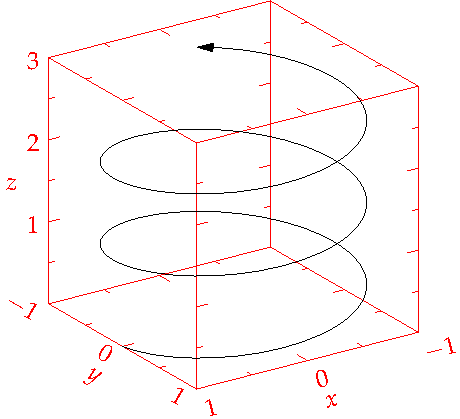
\includegraphics[width=\linewidth]{helix}
    \caption{Superficie, campo y flujo magnético.}
    \label{fig:flujomagnetico}
\end{marginfigure}

El flujo magnético $\phi_m$ a través de una superficie $A$ se calcula de forma análoga al flujo de un campo eléctrico. Siendo $dA$ un elemento de área infinitesimal de dicha superficie y $\hat{n}$ el vector unitario perpendicular a dicho elemento \sidenote{Podemos observar además que, si bien hay dos direcciones normales posibles, su elección es arbitraria y el signo del flujo no depende de dicha elección.}, el flujo queda definido como sigue (siendo su unidad el \emph{Weber} $[Wb]$ que equivale a $[T\cdot m^2]$)

\begin{equation}
\phi_m = \int_{S} \mathbf{\vec{B}}\mathbf{\hat{n}}dA = \int_{S}B_ndA ~ [Wb]~, 
\end{equation}

Dado que el campo magnético es proporcional al número de líneas de campo por unidad de área, el flujo es proporcional al número de líneas que atraviesan dicha superficie. Por lo tanto, si la superficie es un plano de área $A$ y el campo magnético es constante sobre la superficie, el flujo que la atraviesa es

\begin{equation}
\phi_m = \mathbf{\vec{B}}\mathbf{\hat{n}}A = BA\cos{\theta} ~ [Wb]~,
\end{equation}

donde $\theta$ es el ángulo que forman el campo magnético y la normal de la superficie. Frecuentemente, esta aproximación se utiliza para calcular el flujo magnético a través de una superficie rodeada por una bobina con $N$ espiras

\begin{equation}
\phi_m = N\mathbf{\vec{B}}\mathbf{\hat{n}}A = NBA\cos{\theta} ~ [Wb]~.
\end{equation}

\begin{marginfigure}%
    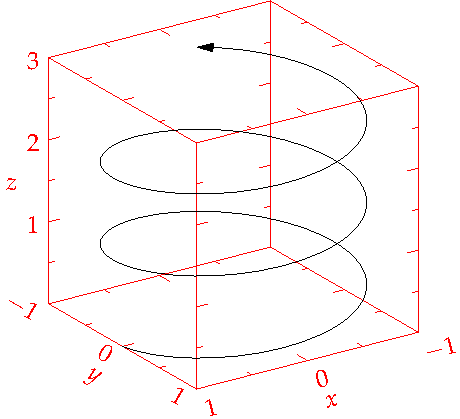
\includegraphics[width=\linewidth]{helix}
    \caption{Flujo magnético a través de una superficie $S$ encerrada por una bobina con $N$ espiras o vueltas.}
    \label{fig:flujomagneticoespira}
\end{marginfigure}

\subsection{FEM Inducida y Ley de Faraday}

Si el flujo magnético a través de un área rodeada por un circuito varía por cualquier motivo, se induce una FEM que es igual en módulo a la variación por unidad de tiempo del flujo que atraviesa dicho circuito:

\begin{equation}
\mathcal{E} = -\displaystyle\frac{d\phi_m}{dt}~[V]~.
\end{equation}

Los campos eléctricos estudiados con anterioridad eran producidos por cargas eléctricas estáticas por lo que su circulación (potencial como $\oint_{C}\mathbf{\vec{E}}\cdot d\mathbf{\vec{l}}$) alrededor de una curva cerrada $C$ era cero. No obstante, el campo eléctrico generador por un campo magnético variable no es conservativo ya que su circulación (potencial) es una FEM inducida por el flujo magnético que atraviesa cualquier superficie $S$ encerrada por $C$ tal y como comentamos anteriormente

\begin{equation}
\mathcal{E} = \oint_{C}\mathbf{\vec{E}_{nc}}\cdot d \mathbf{\vec{l}} = -\displaystyle\frac{d}{dt}\int_{S}\mathbf{\vec{B}}\cdot\mathbf{\hat{n}}dA = -\displaystyle\frac{d\phi_m}{dt}~[V]~.
\end{equation}

\subsection{Ley de Lenz}

\begin{marginfigure}%
    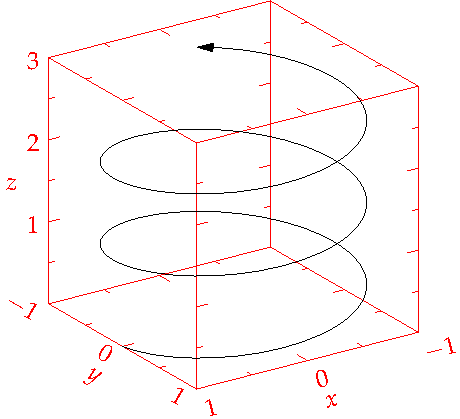
\includegraphics[width=\linewidth]{helix}
    \caption{Ejemplo de la Ley de Lenz.}
    \label{fig:ejemplolenz}
\end{marginfigure}

Cuando se produce una variación del flujo magnético que atraviesa una superficie, el campo magnético debido a la corriente inducida genera un flujo magnético sobre la misma superficie que se opone a dicha variación. Dicho de otro modo, la Ley de Lenz es la responsable del signo negativo en la Ley de Faraday puesto que la FEM y la corriente inducidas poseen una dirección y sentido tal que tienden a oponerse a la variación que las produce.

\subsection{FEM de Movimiento}

La FEM inducida en un conductor que se mueve a través de un campo magnético se denomina FEM de movimiento. El ejemplo más claro es el de una varilla conductora que se desliza a lo largo de dos conductores unidos a una resistencia, todo ello en el seno de un campo magnético uniforme tal y como se muestra en la Figura \ref{fig:femmovimiento}.

\begin{marginfigure}%
    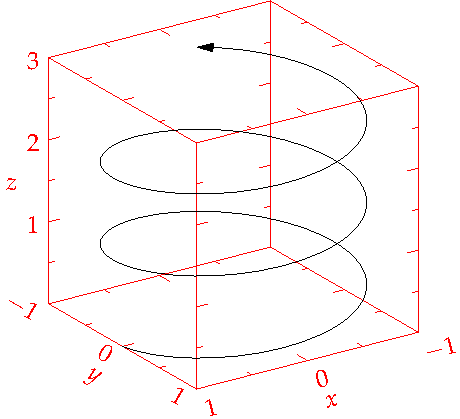
\includegraphics[width=\linewidth]{helix}
    \caption{Varilla conductora deslizante sobre raíles conductores (conectados a una resistencia) en el seno de un campo magnético.}
    \label{fig:femmovimiento}
\end{marginfigure}

En este caso, el área de la superficie $S$ encerrada por el circuito se incrementa cuando la varilla se desplaza a la derecha por lo que el flujo magnético a través de la misma también crece y por ello se induce una FEM en el circuito. Si denominamos $l$ a la distancia entre los raíles y $x$ a la distancia entre el extremo izquierdo de los raíles y la varilla, el área es $lx$ y por lo tanto el flujo es

\begin{equation}
\phi_m = BA = Blx~[Wb].
\end{equation}

Si derivamos respecto al tiempo para obtener la variación del flujo respecto al mismo (teniendo en cuenta que $x$ varía con el tiempo \sidenote{La variación de la longitud $x$ con el tiempo es simplemente la velocidad a la que se desplaza la varilla $v = \displaystyle\frac{dx}{dt}$})

\begin{equation}
\displaystyle\frac{d\phi_m}{dt} = Bl\displaystyle\frac{dx}{dt} = Blv~[V]~,
\end{equation}

podemos deducir que la FEM inducida en el circuito es

\begin{equation}
\mathcal{E} = -\displaystyle\frac{d\phi_m}{dt} = -Blv~[V]
\end{equation}

\subsection{Generadores y Motores}

Un generador de corriente alterna se puede construir mediante una bobina giratoria en el seno de un campo magnético uniforme. Los extremos de la bobina se conectan a un anillo deslizante que gira con la bobina. Cuando la bobina gira por acción mecánica, el flujo magnético a través de ella varía y por lo tanto se induce una FEM en ella. El ángulo formado entre el campo magnético $\mathbf{\vec{B}}$ y la normal de la superficie de la bobina $\mathbf{\hat{n}}$ viene dado por

\begin{marginfigure}%
    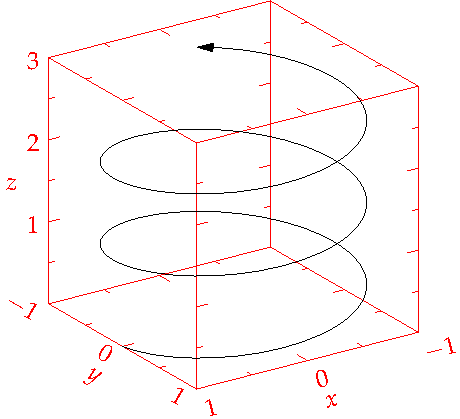
\includegraphics[width=\linewidth]{helix}
    \caption{Generador de corriente alterna en el que una bobina girando con velocidad angular constante en el seno de un campo magnético genera una FEM inducida sinusoidal.}
    \label{fig:generadorac}
\end{marginfigure}

\begin{equation}
\theta = \omega t~[deg]~,
\end{equation}

por lo tanto, el flujo magnético que atraviesa la bobina depende del tiempo y de la velocidad angular de rotación de la misma como sigue

\begin{equation}
\phi_m = NBA\cos{\omega t} = NBA\cos{2\pi f}~[Wb]~.
\end{equation}

Podemos deducir entonces que la FEM producida por la bobina es 

\begin{equation}
\mathcal{E} = - \displaystyle\frac{d\phi_m}{dt} = \omega NBA\sin{\omega t} = \mathcal{E}_{max} \sin{\omega t} ~[V]~,
\end{equation}

donde

\begin{equation}
\mathcal{E}_{max} = \omega NBA~[V]~.
\end{equation}

\subsection{Inductancia}

El flujo magnético generado a través de una bobina por una corriente que circula por la misma es proporcional a la intensidad de corriente según una constante $L~[H]$ \sidenote{La unidad del sistema internacional para la inductancia $L$ es el Henry $[H]$.}

\begin{equation}
\phi_m = LI~[Wb]~,
\end{equation}

esta constante se denomina autoinducción y depende de la geometría de la bobina. Para el caso de un solenoide enrollado determinamos anteriormente que el flujo máximo venía dado por $NBA$, por lo que desarrollando esta igualdad

\begin{equation}
\phi_m = NBA = N(\mu_0 nI)A = \mu_0 n^2 IAl~[H]~,
\end{equation}

ya que el campo magnético es conocido $B=\mu_0 nI$ y el número de vueltas de la bobina también $N=nl$. La constante de proporcionalidad respecto a la intensidad de corriente es la autoinducción y únicamente depende de factores geométricos

\begin{equation}
L = \phi_m / I = \mu_0 n^2 Al~[H]~.
\end{equation}

\subsection{Energía Magnética}

De la misma forma que un condensador almacena energía eléctrica, un inductor almacena energía magnética. La energía almacenada en un inductor que transporta una corriente $I$ es

\begin{equation}
U_m = \displaystyle\frac{1}{2}LI^2~[J]~.
\end{equation}

Esa energía magnética puede ser expresada como

\begin{equation}
U_m = \displaystyle\frac{1}{2}LI^2 = \displaystyle\frac{1}{2}\mu_0n^2Al(\displaystyle\frac{B}{\mu_0 n})^2 = \displaystyle\frac{B}{\mu_0 n}^2Al~[J]~,
\end{equation}

y a partir de la misma podemos derivar la densidad de energía magnética $u_m$ como la energía por unidad de volumen $Al$

\begin{equation}
u_m = \displaystyle\frac{B^2}{2\mu_0}~[J\cdot m^{-3}]~.
\end{equation}

\subsection{Circuitos RL}

\begin{marginfigure}%
    \centering
    \begin{circuitikz}
\draw (0,0)
  to[V=$V_{in}$, invert] (0,2) % The voltage source
  to[R=\(R_1\)] (3,2) % The resistor
  to[L=\(L_1\)] (3,0) % The inductor
  to (0,0); %Inductor One
\end{circuitikz}
    \bigskip
    \caption{Circuito RL básico.}
    \label{fig:circuitorl}
\end{marginfigure}

Un circuito RL (ver Figura \ref{fig:circuitorl}) es todo aquel que contiene una resistencia y un inductor. La aplicación de la regla de las mallas de Kirchoff arroja la siguiente expresión para el circuito

\begin{equation}
\mathcal{E}_0 - IR - L\displaystyle\frac{dI}{dt} = 0
\end{equation}

En el instante inicial, la corriente es nula por lo que $IR$ es cero y la FEM de la batería es igual a la caída de potencial en el inductor. Cuando la corriente comienza a crecer, $IR$ crece y la variación de la corriente con el tiempo disminuye \sidenote{Cuando la inductancia $L$ no es despreciable, $I$ no puede saltar súbitamente de cero a un valor finito sino que $dI/dt$ es finita y por lo tanto la corriente es continua en el tiempo.} hasta que en un tiempo breve, la corriente alcanza un valor positivo $I$. Su variación con el tiempo podemos resolverla separando variables e integrando

\begin{equation}
\displaystyle\frac{dI}{dt} = \mathcal{E} - \displaystyle\frac{IR}{L} \rightarrow \displaystyle\frac{dI}{\mathcal{E}-IR} = \displaystyle\frac{dt}{L}
\end{equation}

\marginnote{Cuanto mayor es la autoinducción $L$ o menor es la resistencia $R$ del circuito, más tiempo es necesario para establecer una fracción determinada de la corriente final $I_0$.}

\begin{equation}
I(t) = \displaystyle\frac{\mathcal{E}}{R}(1 - e^{-\displaystyle\frac{R}{L}t}) = I_0 (1 - e^{-\displaystyle\frac{t}{\tau}})~[A]~,
\end{equation}

donde $I_0$ es el valor máximo o final de la corriente $\mathcal{E/R}~[A]$ cuando $t\rightarrow \infty$ y $\tau$ es la constante de tiempo o tiempo característico del circuito $L/R~[s]$.

\begin{figure*}[h]
    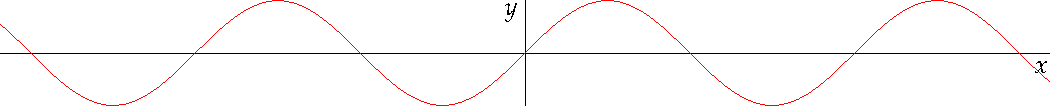
\includegraphics[width=\linewidth]{sine.pdf}%
    \caption{Variación de la intensidad de corriente en función del tiempo en un circuito RL.}%
    \label{fig:fullfig}%
  \end{figure*}


\clearpage

\section{Ondas Electromagnéticas}

\clearpage

\section{Óptica}

\clearpage

\subsection{Sidenotes}\label{sec:sidenotes}
One of the most prominent and distinctive features of this style is the
extensive use of sidenotes.  There is a wide margin to provide ample room
for sidenotes and small figures.  Any \Verb|\footnote|s will automatically
be converted to sidenotes.\footnote{This is a sidenote that was entered
using the \texttt{\textbackslash footnote} command.}  If you'd like to place ancillary
information in the margin without the sidenote mark (the superscript
number), you can use the \Verb|\marginnote| command.\marginnote{This is a
margin note.  Notice that there isn't a number preceding the note, and
there is no number in the main text where this note was written.}

The specification of the \Verb|\sidenote| command is:
\begin{docspec}
  \doccmd{sidenote[\docopt{number}][\docopt{offset}]\{\docarg{Sidenote text.}\}}
\end{docspec}

Both the \docopt{number} and \docopt{offset} arguments are optional.  If you
provide a \docopt{number} argument, then that number will be used as the
sidenote number.  It will change of the number of the current sidenote only and
will not affect the numbering sequence of subsequent sidenotes.

Sometimes a sidenote may run over the top of other text or graphics in the
margin space.  If this happens, you can adjust the vertical position of the
sidenote by providing a dimension in the \docopt{offset} argument.  Some
examples of valid dimensions are:
\begin{docspec}
  \ttfamily 1.0in \qquad 2.54cm \qquad 254mm \qquad 6\Verb|\baselineskip|
\end{docspec}
If the dimension is positive it will push the sidenote down the page; if the
dimension is negative, it will move the sidenote up the page.

While both the \docopt{number} and \docopt{offset} arguments are optional, they
must be provided in order.  To adjust the vertical position of the sidenote
while leaving the sidenote number alone, use the following syntax:
\begin{docspec}
  \doccmd{sidenote[][\docopt{offset}]\{\docarg{Sidenote text.}\}}
\end{docspec}
The empty brackets tell the \Verb|\sidenote| command to use the default
sidenote number.

If you \emph{only} want to change the sidenote number, however, you may
completely omit the \docopt{offset} argument:
\begin{docspec}
  \doccmd{sidenote[\docopt{number}]\{\docarg{Sidenote text.}\}}
\end{docspec}

The \Verb|\marginnote| command has a similar \docarg{offset} argument:
\begin{docspec}
  \doccmd{marginnote[\docopt{offset}]\{\docarg{Margin note text.}\}}
\end{docspec}

\subsection{References}
References are placed alongside their citations as sidenotes,
as well.  This can be accomplished using the normal \Verb|\cite|
command.\sidenote{The first paragraph of this document includes a citation.}

The complete list of references may also be printed automatically by using
the \Verb|\bibliography| command.  (See the end of this document for an
example.)  If you do not want to print a bibliography at the end of your
document, use the \Verb|\nobibliography| command in its place.  

To enter multiple citations at one location,\cite{Tufte2006,Tufte1990} you can
provide a list of keys separated by commas and the same optional vertical
offset argument: \Verb|\cite{Tufte2006,Tufte1990}|.  
\begin{docspec}
  \doccmd{cite[\docopt{offset}]\{\docarg{bibkey1,bibkey2,\ldots}\}}
\end{docspec}

\section{Figures and Tables}\label{sec:figures-and-tables}
Images and graphics play an integral role in Tufte's work.
In addition to the standard \docenv{figure} and \docenv{tabular} environments,
this style provides special figure and table environments for full-width
floats.

Full page--width figures and tables may be placed in \docenv{figure*} or
\docenv{table*} environments.  To place figures or tables in the margin,
use the \docenv{marginfigure} or \docenv{margintable} environments as follows
(see figure~\ref{fig:marginfig}):

\begin{marginfigure}%
  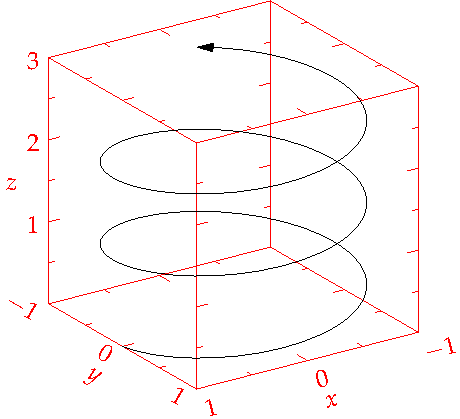
\includegraphics[width=\linewidth]{helix}
  \caption{This is a margin figure.  The helix is defined by 
    $x = \cos(2\pi z)$, $y = \sin(2\pi z)$, and $z = [0, 2.7]$.  The figure was
    drawn using Asymptote (\url{http://asymptote.sf.net/}).}
  \label{fig:marginfig}
\end{marginfigure}
\begin{Verbatim}
\begin{marginfigure}
  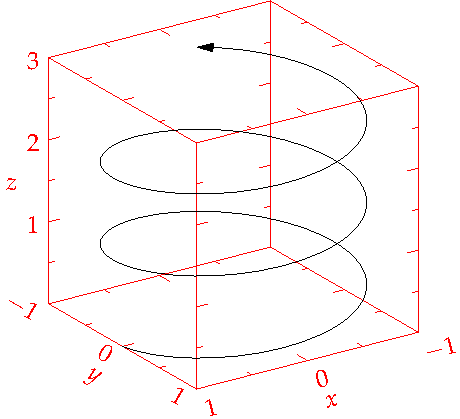
\includegraphics{helix}
  \caption{This is a margin figure.}
\end{marginfigure}
\end{Verbatim}

The \docenv{marginfigure} and \docenv{margintable} environments accept an optional parameter \docopt{offset} that adjusts the vertical position of the figure or table.  See the ``\nameref{sec:sidenotes}'' section above for examples.  The specifications are:
\begin{docspec}
  \doccmd{begin\{marginfigure\}[\docopt{offset}]}\\
  \qquad\ldots\\
  \doccmd{end\{marginfigure\}}\\
  \mbox{}\\
  \doccmd{begin\{margintable\}[\docopt{offset}]}\\
  \qquad\ldots\\
  \doccmd{end\{margintable\}}\\
\end{docspec}

Figure~\ref{fig:fullfig} is an example of the \Verb|figure*|
environment and figure~\ref{fig:textfig} is an example of the normal
\Verb|figure| environment.

\begin{figure*}[h]
  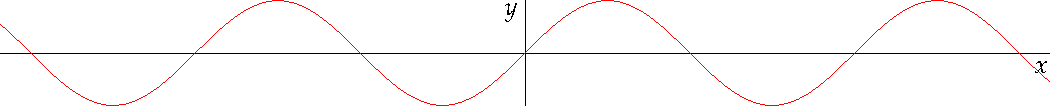
\includegraphics[width=\linewidth]{sine.pdf}%
  \caption{This graph shows $y = \sin x$ from about $x = [-10, 10]$.
  \emph{Notice that this figure takes up the full page width.}}%
  \label{fig:fullfig}%
\end{figure*}

\begin{figure}
  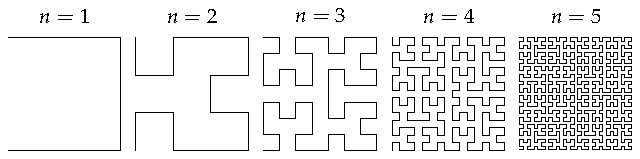
\includegraphics{hilbertcurves.pdf}
%  \checkparity This is an \pageparity\ page.%
  \caption{Hilbert curves of various degrees $n$.
  \emph{Notice that this figure only takes up the main textblock width.}}
  \label{fig:textfig}
  %\zsavepos{pos:textfig}
  \setfloatalignment{b}
\end{figure}

Table~\ref{tab:normaltab} shows table created with the \docpkg{booktabs}
package.  Notice the lack of vertical rules---they serve only to clutter
the table's data.

\begin{table}[ht]
  \centering
  \fontfamily{ppl}\selectfont
  \begin{tabular}{ll}
    \toprule
    Margin & Length \\
    \midrule
    Paper width & \unit[8\nicefrac{1}{2}]{inches} \\
    Paper height & \unit[11]{inches} \\
    Textblock width & \unit[6\nicefrac{1}{2}]{inches} \\
    Textblock/sidenote gutter & \unit[\nicefrac{3}{8}]{inches} \\
    Sidenote width & \unit[2]{inches} \\
    \bottomrule
  \end{tabular}
  \caption{Here are the dimensions of the various margins used in the Tufte-handout class.}
  \label{tab:normaltab}
  %\zsavepos{pos:normaltab}
\end{table}

\section{Full-width text blocks}

In addition to the new float types, there is a \docenv{fullwidth}
environment that stretches across the main text block and the sidenotes
area.

\begin{Verbatim}
\begin{fullwidth}
Lorem ipsum dolor sit amet...
\end{fullwidth}
\end{Verbatim}

\begin{fullwidth}
\small\itshape\lipsum[1]
\end{fullwidth}

\section{Typography}\label{sec:typography}

\subsection{Typefaces}\label{sec:typefaces}
If the Palatino, \textsf{Helvetica}, and \texttt{Bera Mono} typefaces are installed, this style
will use them automatically.  Otherwise, we'll fall back on the Computer Modern
typefaces.

\subsection{Letterspacing}\label{sec:letterspacing}
This document class includes two new commands and some improvements on
existing commands for letterspacing.

When setting strings of \allcaps{ALL CAPS} or \smallcaps{small caps}, the
letter\-spacing---that is, the spacing between the letters---should be
increased slightly.\cite{Bringhurst2005}  The \Verb|\allcaps| command has proper letterspacing for
strings of \allcaps{FULL CAPITAL LETTERS}, and the \Verb|\smallcaps| command
has letterspacing for \smallcaps{small capital letters}.  These commands
will also automatically convert the case of the text to upper- or
lowercase, respectively.

The \Verb|\textsc| command has also been redefined to include
letterspacing.  The case of the \Verb|\textsc| argument is left as is,
however.  This allows one to use both uppercase and lowercase letters:
\textsc{The Initial Letters Of The Words In This Sentence Are Capitalized.}



\section{Installation}\label{sec:installation}
To install the Tufte-\LaTeX\ classes, simply drop the
following files into the same directory as your \texttt{.tex}
file:
\begin{quote}
  \ttfamily
  tufte-common.def\\
  tufte-handout.cls\\
  tufte-book.cls
\end{quote}

% TODO add instructions for installing it globally



\section{More Documentation}\label{sec:more-doc}
For more documentation on the Tufte-\LaTeX{} document classes (including commands not
mentioned in this handout), please see the sample book.

\section{Support}\label{sec:support}

The website for the Tufte-\LaTeX\ packages is located at
\url{http://code.google.com/p/tufte-latex/}.  On our website, you'll find
links to our \smallcaps{svn} repository, mailing lists, bug tracker, and documentation.

\bibliography{sample-handout}
\bibliographystyle{plainnat}



\end{document}